% Delta-KB field-image samples (real Bugwood photographs, geo-tagged).
\begin{figure}[t]
\centering
\begin{subfigure}{0.235\textwidth}\centering
  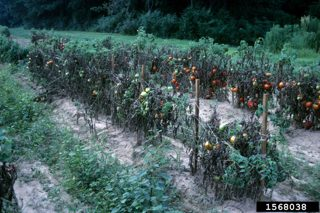
\includegraphics[width=\linewidth]{figures/delta_early_blight.jpg}
  \caption{Early Blight}
\end{subfigure}\hfill
\begin{subfigure}{0.235\textwidth}\centering
  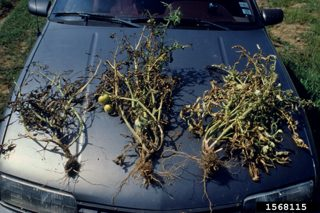
\includegraphics[width=\linewidth]{figures/delta_southern_blight.jpg}
  \caption{Southern Blight}
\end{subfigure}\\[2pt]
\begin{subfigure}{0.235\textwidth}\centering
  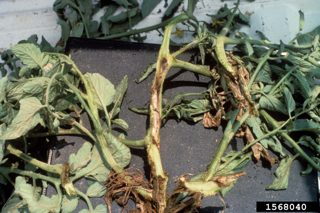
\includegraphics[width=\linewidth]{figures/delta_bacterial_canker.jpg}
  \caption{Bacterial Canker}
\end{subfigure}\hfill
\begin{subfigure}{0.235\textwidth}\centering
  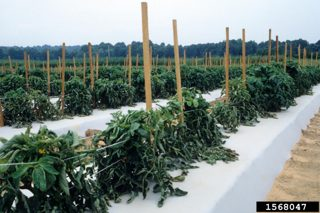
\includegraphics[width=\linewidth]{figures/delta_cucumber_mosaic.jpg}
  \caption{Cucumber Mosaic}
\end{subfigure}
\caption{Representative geo-tagged \bugwood{} field photographs (Tomato) that
the swarm captions to extract per-(disease, state) \emph{deltas}. Unlike
studio benchmark images, these carry realistic clutter, lighting, and
viewpoint---the distribution the encoder is tuned on and the deltas describe.}
\label{fig:delta-samples}
\end{figure}
